\documentclass{ximera}  
\title{If/Else Statements}  
\begin{document}  
\begin{abstract}  
We introduce if/else statements in Python.
\end{abstract}  
\maketitle

\section{If/Else}

In an earlier section we saw that in order to compute the absolute value of a real number $x$, we first needed to determine if it satisfied a certain condition, namely, is it the case that $x>0$? The answer to this question then determines the set of instructions to follow. We can reformulate our algorithm for computing $|x|$ as two statements in the following way:

For any real number $x$, if $x>0$, then $|x|=x$. Else (or otherwise), $|x|=-x$.

The `if' portion of the statement explains what to do if the given condition is satisfied, while the `else' portion explains what to do if the given condition is not satisfied. This can be easily mapped to the flowchart for computing $|x|$ below.

\begin{center}
	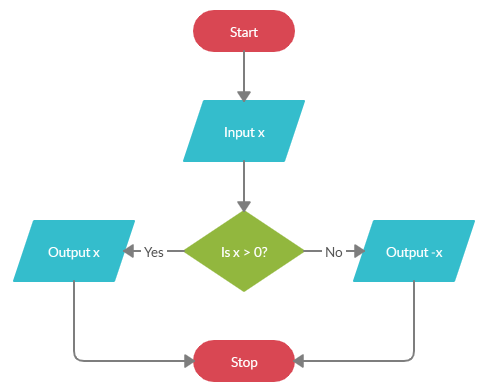
\includegraphics{absalgo.png}
\end{center}

In Python we can implement this short algorithm using the following syntax:

\begin{verbatim}
if (condition):
        code1
else:
        code2
\end{verbatim}

The term \verb|condition| indicates the condition we wish to check. If the condition evaluates to \verb|True|, then the instructions given by \verb|code1| are followed. If the condition evaluates to \verb|False|, then the instructions given by \verb|code2| are followed. Using the template above, we can now write the necessary Python code to compute $|x|$.

\begin{verbatim}
if x > 0:
        abs = x
else:
        abs = -x
\end{verbatim}

The code above creates a variable \verb|abs| that is assigned the absolute value of $x$ for any given $x$. The SageCell below shows how to use this code in practice.

\begin{sageCell}
x = -3            # change this value and evaluate the cell to compute |x| for other x values

if x > 0:
	abs = x
else:
	abs = -x

print(abs)        # this line prints the value of abs to the screen to show that the variable has been assigned the correct value
\end{sageCell}

Note that in Python, whitespace (indentation) determines which lines of code belong to a particular code block. For example, the following code differs from that in the SageCell above in that the \verb|print| statement is only evaluated if $x\leq 0$.

\begin{sageCell}
x = -3

if x > 0:
	abs = x
else:
	abs = -x
        print(abs)
\end{sageCell}

The examples above show how a flowchart with a decision compartment can be translated to Python code and vice versa. With enough practice one shoud be able to translate between the two. Eventually, with enough experience, one can start coding without explicitly drawing a flowchart each time.

Below we give examples of how to use the basic if/else form to handle cases where multiple decisions are needed of if a decision has more than two outcomes. 




\begin{problem}
\end{problem}

\begin{problem}
\end{problem}

\end{document}
